\documentclass[10pt]{article}
\usepackage{icmlko}

\icmlmeta{IP 파운데이션 월드모델}{235}{비어 있는 것이 무엇이냐가 전부다}{노트 234가 관측률로 판을 갈랐더니 모바일 +0.21 · 애니 −0.05 였다. 어느 축이 비었는지 보니 두 이상이 한 번에 풀린다}

\begin{document}

\twocolumn[
\icmlheader

\begin{abstract}
노트 234가 유보 행을 관측률로 갈라 두 판을 적고 \textbf{모바일 $+$0.21 ·
애니 $-$0.05} 라는 반대 부호를 남겼다. \textbf{어느 축이 비어 있는지}를
봤더니 둘 다 한 번에 풀린다. \textbf{모바일에서 두 쪽을 가르는 것은 검색
축 하나뿐이다} --- 대입 쪽 150건의 검색 관측률이 \textbf{1.3\%} 이고 관측
쪽 291건은 \textbf{90.4\%} 다. 나머지 축은 두 쪽이 거의 같다(타깃 폭
98.7 대 100.0, 위키 0.0 대 9.6, 미디어 푸시 0.7 대 1.4). \textbf{그리고
그 검색이 모바일의 제일 센 축이다} --- 모멘텀 $+$0.323 · 수준 $+$0.305 ·
변동 $+$0.229 로, 다음이 타깃 폭 $+$0.103 이다. \textbf{그러니 대입 쪽
150건은 ``덜 채워진 행''이 아니라 ``제일 센 축이 없는 행''이고, 그래서
$+$0.21 만큼 못 맞힌다.} 애니는 정반대 기전으로 반대 부호가 난다. 두
쪽을 가르는 것이 \textbf{위키 축}(0.3\% 대 76.3\%)과 장소 노출(1.3\% 대
39.5\%)인데, \textbf{그 위키 축들이 라벨과 음의 상관이다} --- 수준
$-$0.176 · 변동 $-$0.195 · 피크 $-$0.187. \textbf{관측 쪽이 해로운 축을
더 갖고 있어서 오히려 못 맞힌다.} 그러면 결론이 하나로 모인다 ---
\textbf{관측률 격차는 ``얼마나 채웠나''가 아니라 ``어느 축이 비었나''다.}
노트 234가 관측률을 하나의 수로 쓴 것 자체가 아직 거친 것이었다. 그리고
곧바로 쓸 데가 있다 --- 노트 220이 모바일 검색 천장을 $+$0.0669 로 쟀고
노트 221이 덮음을 54.2\% $\to$ 60.1\% 로 올렸는데, \textbf{남은 40\% 가
바로 이 150건이고 그것을 채우면 그 천장에 닿는다.}
\end{abstract}
]

\begin{figure*}[t]
\centering
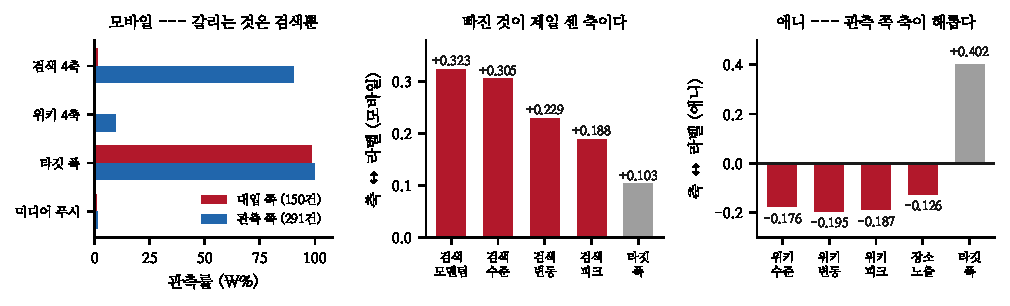
\includegraphics[width=\textwidth]{figs/whichaxis.pdf}
\caption{왼쪽 --- 모바일에서 갈리는 것은 검색뿐. 가운데 --- 그 검색이
제일 센 축. 오른쪽 --- 애니는 관측 쪽 축이 해롭다.}
\end{figure*}

\section{모바일 --- 갈리는 것은 검색뿐}

\begin{table}[t]
\centering\tsize
\caption{모바일 유보 441. 두 쪽의 축별 관측률.}
\begin{tabular}{lrrr}
\toprule
& 대입 쪽(150) & 관측 쪽(291) & 차 \\
\midrule
\textbf{검색 4축} & \textbf{1.3\%} & \textbf{90.4\%} & \textbf{$+$89.1} \\
위키 4축 & 0.0\% & 9.6\% & $+$9.6 \\
타깃 폭 & 98.7\% & 100.0\% & $+$1.3 \\
미디어 푸시 & 0.7\% & 1.4\% & $+$0.7 \\
\bottomrule
\end{tabular}
\end{table}

\claimx{\textbf{두 쪽을 가르는 것은 검색 축 하나뿐이다}(89.1\%p). 나머지
축은 두 쪽이 거의 같다.}{\textbf{그러니 ``관측률 0.7 로 자른다''는 것이
사실 ``검색이 있느냐로 자른다''였다} --- 노트 234가 만든 렌즈가
실제로는 축 하나를 재고 있었다.}

\begin{table}[t]
\centering\tsize
\caption{모바일에서 축 $\leftrightarrow$ 라벨(관측된 행만).}
\begin{tabular}{lr}
\toprule
\textbf{검색 모멘텀} & \textbf{$+$.323} \\
\textbf{검색 수준} & \textbf{$+$.305} \\
검색 변동 & $+$.229 \\
검색 피크 & $+$.188 \\
\midrule
타깃 폭 & $+$.103 \\
\bottomrule
\end{tabular}
\end{table}

\claimx{\textbf{그 검색이 모바일의 제일 센 축이다} --- 상위 넷이 전부
검색이고 다음이 타깃 폭 $+$0.103 이다.}{\textbf{대입 쪽 150건은 ``덜
채워진 행''이 아니라 ``제일 센 축이 없는 행''이다.} 그래서 $+$0.21 만큼
못 맞힌다 --- 그 크기가 이상한 것이 아니라 당연하다.}

\section{애니 --- 관측 쪽 축이 해롭다}

\begin{table}[t]
\centering\tsize
\caption{애니 유보 606. 두 쪽을 가르는 축과 그 상관.}
\begin{tabular}{lrrr}
\toprule
& 대입 쪽 & 관측 쪽 & $\leftrightarrow$라벨 \\
\midrule
\textbf{위키 수준} & 0.3\% & 76.3\% & \textbf{$-$.176} \\
\textbf{위키 변동} & 0.3\% & 76.3\% & \textbf{$-$.195} \\
\textbf{위키 피크} & 0.3\% & 76.3\% & \textbf{$-$.187} \\
장소 노출 & 1.3\% & 39.5\% & $-$.126 \\
\midrule
타깃 폭 & 96.2\% & 100.0\% & $+$.402 \\
\bottomrule
\end{tabular}
\end{table}

\claimx{\textbf{애니에서 두 쪽을 가르는 축들이 라벨과 음의 상관이다}
(위키 셋이 $-$0.18$\sim$$-$0.20, 장소 노출 $-$0.13). \textbf{관측 쪽이
해로운 축을 더 갖고 있어서 오히려 못 맞힌다.}}{노트 234의 $-$0.05 가
설명된다 --- \textbf{이상 현상이 아니라 축 하나가 방향을 뒤집은
것이다.}}

\claimx{\textbf{위키 축이 애니에서 음수라는 것 자체가 새 사실이다.}
노트 149가 위키 조회수를 ``네이버 검색이 0\% 인 만화 · 세계애니를
채운다''고 넣었는데, \textbf{애니에서는 넣을수록 해롭다.}}{다만 이
노트는 그것을 \emph{관측}으로만 적는다 --- 축을 끄는 것은 판정치로
정하는 일이고 노트 220의 천장부터 재야 한다.}

\section{결론}

\claimx{\textbf{관측률 격차는 ``얼마나 채웠나''가 아니라 ``어느 축이
비었나''다.} 같은 0.7 자름이 모바일에서는 ``검색이 있느냐''이고
애니에서는 ``위키가 있느냐''인데, 그 둘의 상관 부호가 반대라 판에서
서로 지운다.}{\textbf{노트 234가 관측률을 하나의 수로 쓴 것 자체가 아직
거친 것이었다} --- 렌즈를 만들자마자 그 렌즈도 평균이었다.}

\begin{table}[t]
\centering\tsize
\caption{곧바로 쓸 데.}
\begin{tabular}{ll}
\toprule
노트 220 & 모바일 검색 천장 $+$0.0669 \\
노트 221 & 덮음 54.2\% $\to$ 60.1\% 로 올림 \\
\textbf{이 노트} & \textbf{남은 40\% 가 그 150건이다} \\
\bottomrule
\end{tabular}
\end{table}

\begin{table}[t]
\centering\tsize
\caption{남은 것.}
\begin{tabular}{ll}
\toprule
\textbf{모바일 검색} & 150건을 채우면 천장에 닿나 \\
\textbf{애니 위키} & 음수 축 --- 천장부터 잴 것 \\
자름 대신 축 & 관측률 말고 축별로 가를 것 \\
\bottomrule
\end{tabular}
\end{table}

첫 줄이 이 사이클에서 처음으로 \emph{수집}을 가리키는 자리이고, 이번에는
무엇을 왜 모으는지가 셋 다 명시돼 있다 --- \textbf{어느 행}(모바일 유보
150건과 그에 대응하는 학습 행), \textbf{어느 축}(네이버 검색 넷),
\textbf{얼마짜리}(노트 220의 천장 $+$0.0669, 그중 아직 안 닿은 몫).
\textbf{노트 221이 검색어 추출기 버그를 고쳐 덮음을 6\%p 올렸는데 그때는
남은 것이 무엇인지 몰랐다} --- 지금은 안다. 남은 모바일 미수집은 제목이
순 영문이거나 한글이 두 자 미만인 것들이고, 노트 221에서 게임 322건에
대해 미룬 \emph{음역} 문제와 같은 것이다.

\end{document}
